\section{Comparative Study to Existing Designs} \label{sec:res}

The proposed latch designs were implemented using the 1.05V 32nm PTM library \cite{PTM} and simulated in HSPICE. All transistor widths for all designs were set to minimum size which is 80nm for PMOS and 40nm for NMOS. All designs were operated at 1 Ghz. We compared the HRDNUT and TNU-latch to existing SEU and DNU tolerant designs. We did not compare to other TNU tolerant designs since no other designs are known to exist. For the analysis, we compared to the following SEU tolerant latches: DICE \cite{DICE}, FERST \cite{FERST} and HIPER \cite{HIPER}. Additionally, we compared to the following DNU tolerant designs: DNCS \cite{DNCS}, Interception \cite{Inter}, HSMUF \cite{HSMUF} and DONUT \cite{DONUT}. All transistors for the implemented latches were set to minimum width and length except for the designs that use a C-element with a weak keeper. In these designs the C-element's PMOS width was set to 320nm and the NMOS width was set to 160nm and the weak keeper was sized to be at minimum width. The C-element was sized so that the output driving strength did not allow the keeper to drive the output to an erroneous value in the event of an error. 

\begin{table*}[t]
	\begin{center}
		\caption{SPICE Simulations of Existing Latches using the 1.05V 32nm PTM library }
		\label{table:rtable}
		\begin{tabular}{|m{7em}|m{3.5em}|m{3em}|m{3.5em}|m{2em}|m{3.5em}|m{2em}|}
			\hline
			Latch & DNU\newline Immune & DNU\newline Robust & TNU\newline Immune & Power ($\mu$W) & D-\textgreater Q Delay (ps) & Area (UST)\\ 
			\hline
			DICE & No & No & No & 1.332 & 8.145 & 16 \\
			\hline
			FERST & No & No & No & 3.178 & 31.648 & 60 \\
			\hline
			HIPER & No & No & No & 1.292 & 2.221 & 27 \\
			\hhline{|=|=|=|=|=|=|=|}
			DNCS & Yes & No & No & 4.948 & 22.486 & 61 \\
			\hline
			\cite{Inter} & Yes & No & No & 5.606 & 79.168 & 89 \\
			\hline
			HSMUF & Yes & No & No & 1.871 & 1.0626 & 51 \\
			\hline
			HSMUF (Keeper) & Yes & No & No & 3.787 & 3.945 & 78 \\
			\hhline{|=|=|=|=|=|=|=|}
			DONUT \cite{DONUT} & Yes & Yes & No & 4.021 & 14.722 & 54 \\ 
			\hline
			DONUT-M & Yes & Yes & No & 2.760 & 8.421 & 72\\
			\hline
			HRDNUT (Proposed) & Yes & Yes & No & 2.450 & 2.310 & 66 \\
			\hline
			TNU-Latch & Yes & No & Yes & 3.899 & 46.89 & 123 \\
			\hline
		\end{tabular}
	\end{center}
\end{table*}
\raggedbottom

We measured the propagation delay, average power consumption, critical charge and area of all designs. We then categorized the designs based on the number of errors they can tolerate and if they are DNU-robust. The delay for each design was calculated based on the difference between the time that input \textit{D} is at $0.5*V_{DD}$ and the output at the same point (D-\textgreater Q delay). The average power was calculated over a 200 ns duration when the latch is error-free. All latches tested do not have a critical charge in a conventional sense. Specifically, it is the number of injected pulses rather than the magnitude that greatly contributes to the SEU, DNU or TNU tolerance of the design. We attempted to find the charge value for this to occur through HSPICE simulation of injected charges up to 1 pC and found that the latches did not flip. Waveforms for the HRDNUT and TNU-Latch are given in Fig. [cite figures]. For the calculation of the area, the unit size transistor (UST) metric as adopted in \cite{DNCS} was used. This metric quantifies the expected area based the total transistor area divided by the unit size. For this case, the unit size was set to be 40 nm. Table \ref{table:rtable} gives the results of the simulation.

\begin{figure}[!htbp]
	\centering
	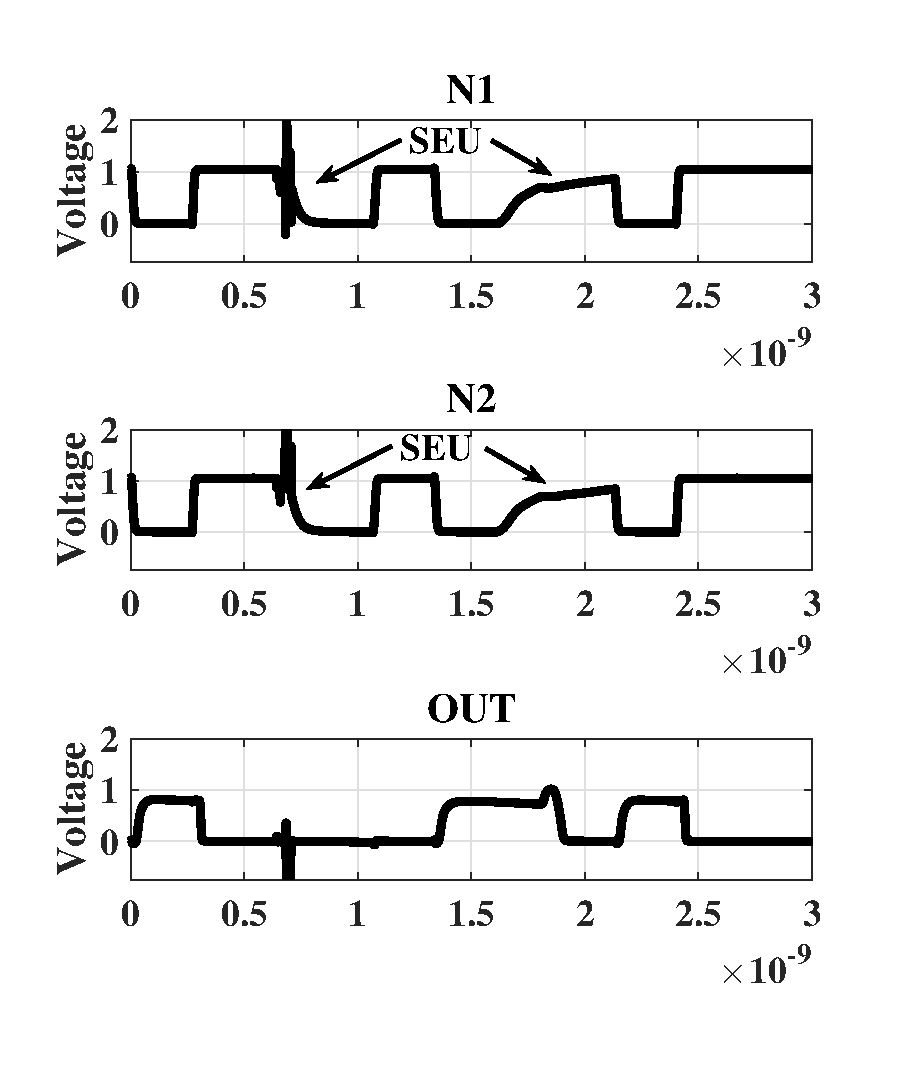
\includegraphics[width=0.55\linewidth]{Figures/DNULargeCharge}
	%where an .eps filename suffix will be assumed under latex, 
	%and a .pdf suffix will be assumed for pdflatex; or what has been declared
	%via \DeclareGraphicsExtensions.
	\caption{Simulation of the HRDNUT for a charge of 1 pC.}
	\label{DNULarge_fig}
\end{figure}

\begin{figure}[!htbp]
	\centering
	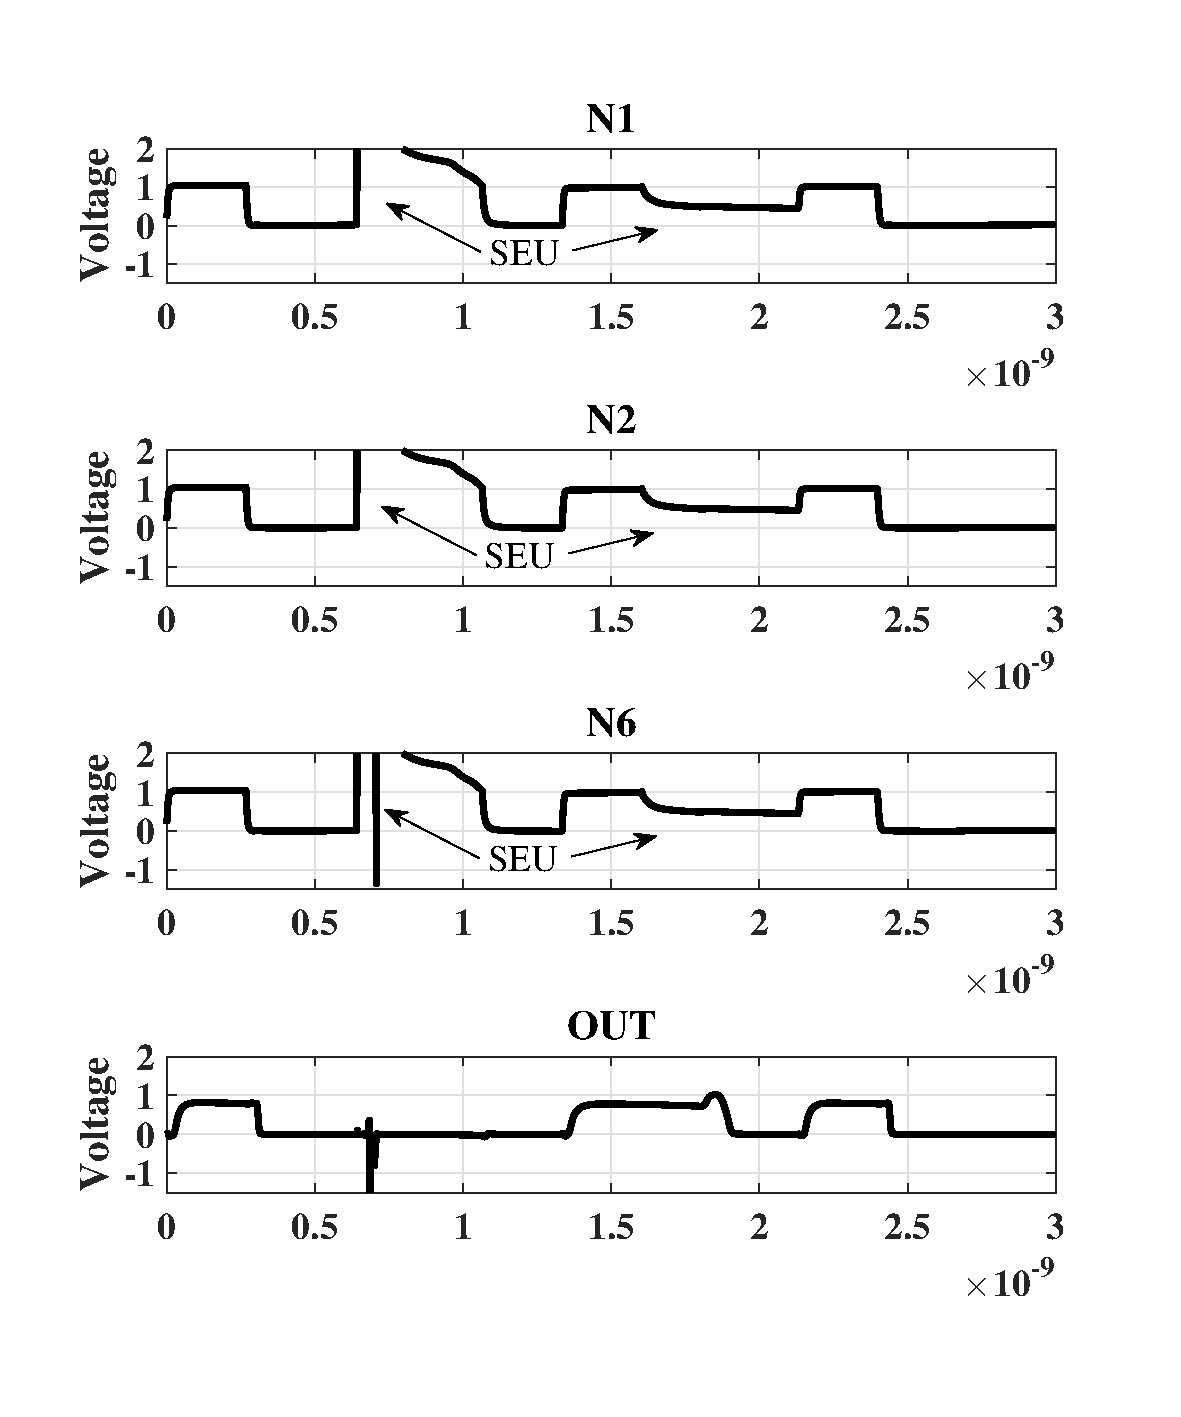
\includegraphics[width=0.75\linewidth]{Figures/largechargetnu}
	%where an .eps filename suffix will be assumed under latex, 
	%and a .pdf suffix will be assumed for pdflatex; or what has been declared
	%via \DeclareGraphicsExtensions.
	\caption{Simulation of the TNU-Latch for a charge of 1 pC.}
	\label{TNULarge_fig}
\end{figure}

According to Table \ref{table:rtable}, the DNU robust designs tested were the two DONUT latches and the HRDNUT. In comparison to the improved DONUT-M latch, the HRDNUT had similar robustness with 11.3\% lower power consumption, 8.33\% fewer transistors and a 72.5\% lower propagation delay. Furthermore, when the HRDNUT was compared to the HSMUF with a keeper, it consumed substantially less power with a lower area and delay. Considering the compared latches, it can be observed that the HRDNUT is the best option for clock gating applications due to DNU robustness and lower power, delay and area overheads.

In addition to the HRDNUT, the TNU-Latch was also compared to many existing designs. While the TNU-Latch does have the highest overhead, it is to be expected due to the additional circuitry that TNU tolerance requires. Compared to the HRDNUT, the TNU-Latch consumes approximately 40\% more power while costing about 2X more area and 20X more delay. The increase in delay is manageable since it is still in the pico-seconds (ps) range which allows the latch to be driven at any commonly used frequency. Additionally, the TNU-Latch still has less delay than the DNU tolerant interception latch \cite{Inter}. Lastly, compared to all other designs, the TNU-Latch is the only latch that provides full TNU resiliency.